\label{chapter:conceitos}
Este capítulo tem como objetivo apresentar as principais conceitos e definições que serão utilizados para o entendimento e desenvolvimento deste trabalho. 


%----------------------------------
% Sistemas Embarcados
%----------------------------------
\section{Sistemas Embarcados}%ok

De acordo com~\citeonline{VAHID:2001} um sistema embarcado é um sistema computacional desenvolvido para um propósito específico, que em contraposição a sistemas de propósito geral, realiza apenas uma tarefa específica. Existem certas características (exemplo, restrição de memória e tempo de execução) que distinguem um sistema embarcado dos demais, que apesar de nem sempre serem atendidas, servem de referência para a classificação de tais sistemas. Sistemas embarcados geralmente realizam apenas uma atividade repetidas vezes, contam com restrições mais apertadas que um sistema normal, são reativos e muitas vezes funcionam em tempo real. Estes sistemas geralmente fazem parte de sistemas maiores, e quase sempre funcionam sem o conhecimento do usuário.

Dispositivos como \textit{smartphones} e computadores pessoais, são compostos por diversos sistemas embarcados que realizam apenas uma função, mas que quando estão juntos passam a realizar diversas atividades, passando a ser classificado como um sistema de propósito geral. Um exemplo de um sistema embarcado que faz parte de um sistema maior seria a placa de rede de um smartphone~\cite{qualcomm_2017}, que por si só é um sistema que apenas recebe e envia dados através de uma rede sem fio, mas que quando contextualizado em um smartphone possibilita o acesso a internet, o que promove a realização de diversas atividades disponíveis online, como acesso à redes sociais ou a reprodução de vídeos~\cite{VAHID:2001}.

%Diante do surgimento da Internet das Coisas (IoT, em inglês), diversos sistemas embarcados capazes de realizar comunicações 

%Este trabalho irá utilizar diversos sistemas embarcados durante o desenvolvimento de seu protótipo, que permitirão que a luva Hand.io atinja um

%\todo[inline]{Falar sobre IoT}

\subsection{Restrições de um Sistema Embarcado} %OK

Um sistema embarcado geralmente trabalha em condições restritas nas quais certas métricas devem ser cumpridas para que seu funcionamento se dê de maneira eficiente. \citeonline{marwedel:2011} define uma série de métricas utilizadas para medir a eficiência de um dado sistema como: consumo energético, eficiência em tempo de execução, tamanho de código, peso e custo. Em alguns casos existem situações onde estas métricas entram em conflito, neste caso cabe ao projetista do sistema definir qual a melhor configuração abrindo mão de certas funcionalidades para melhor atender as necessidades da aplicação.

O consumo de energia em um sistema embarcado muitas vezes é limitado devido à tecnologia atual de baterias e ao tipo do circuito utilizado. Circuitos Integrados de Aplicações Específicas (ASICs, em inglês) tendem a ter uma eficiência energética muito superior aos demais, no entanto abrem mão de flexibilidade no desenvolvimento do software, circuitos reconfiguráveis como os Arranjos de Portas Programáveis em Campo (FPGAs, em inglês) tem sua eficiência energética inferior aos ASICs, mas oferecem uma flexibilidade de desenvolvimento muito maior apesar de serem limitados pelo tamanho dos circuitos reconfiguráveis disponíveis~\cite{marwedel:2011}.

A limitação entre flexibilidade e eficiência também se aplica aos processadores. Processadores desenvolvidos especificamente para processamento de sinais analógicos, por exemplo, são exponencialmente mais eficientes energeticamente que processadores de propósito geral, que contam com a pior eficiência energética dentre os circuitos apresentados, mas permitem uma grande gama de possibilidades durante o desenvolvimento do sistema~\cite{marwedel:2011}.

As limitações em tempo de execução devem ser reduzidas ao máximo para aproveitar o hardware disponível da melhor maneira possível. Problemas acarretados por compiladores que geram binários que não utilizam todo o potencial da arquitetura devem ser corrigidos a fim de eliminar desperdícios de instruções por ciclo de processamento~\cite{marwedel:2011}.

O tamanho do código e as limitações em espaço de armazenamento são um desafio recorrente no mundo dos sistemas embarcados. Em diversas aplicações onde não existe a possibilidade de carregamento dinâmico de dados, como ocorrem nos \textit{smartphones}, todos os dados devem ser armazenados na memória limitada dos chips, como nos casos de \textit{Systems on a Chip} (SoC), nos quais todos os componentes de processamento de dados se encontram em um único chip. Nesse tipo de situação onde o espaço se torna um recurso precioso é necessário um cuidado maior durante a construção do código que será executado na plataforma. Tal limitação pode ser contornada com a utilização de memórias \textit{flash}, mas em certas aplicações devido à outras limitações este tipo de recurso pode não estar disponível~\cite{marwedel:2011}.

O peso dos componentes pode ser o fator decisivo na aplicação de um sistema embarcado, existem situações onde o sistema deve ser portátil, logo um peso elevado acabaria por dificultar o manuseio do protótipo. Nestes casos o projetista deve ter preferência pelos componentes de tamanho mais reduzido possível~\cite{marwedel:2011}.

Em sistemas voltados para o mercado de consumo onde existe um orçamento limitado para o desenvolvimento do sistema, o custo passa a ser uma métrica crucial para o projeto, componentes que não melhoram de maneira significativa a eficiência do pior caso do sistema devem ser descartados afim de reduzir o consumo total de energia. Os requisitos da aplicação devem ser cumpridos utilizando o menor número de componentes possível e com os componentes mais baratos possíveis desde que não comprometam a qualidade do produto final. \cite{marwedel:2011}

%A luva Hand.io contará com diversas restrições em seu protótipo devido à natureza da luva. Por ser uma peça de roupa, se espera que seu peso seja reduzido.

Muitas vezes quando um sistema é desenvolvido em um ambiente com recursos limitados, se faz necessária a utilização de modelos formais para garantir que os recursos disponíveis sejam utilizados da melhor maneira possível. Geralmente o tamanho de código e o tamanho físico de um componente estão em conflito direto com o seu desempenho, o que pode gerar problemas quando um sistema embarcado precisa reagir em tempo real. Modelos formais contam com certos índices de desempenho que podem ser medidos com valores numéricos, o que permite aos desenvolvedores realizar otimizações precisas nas escolha componentes que serão utilizados em um projeto. \citeonline{edwards:1997} 

\subsection{Sistemas de Tempo Real} %OK

Conforme~\citeonline{BUTTAZZO:2011}, um sistema em tempo real deve ter o tempo do sistema medido utilizando a mesma escala de tempo do mundo real, isto ocorre pelo fato de que o sistema deve ter ciência do ambiente no qual ele irá operar. 
% Sistemas em tempo real geralmente contam com uma definição errônea do seu funcionamento, que diz que um sistema em tempo real deve reagir à estímulos externos com uma certa rapidez e que apenas tendo sido este requisito atendido é o suficiente para que o sistema receba tal classificação. 
% Entretanto, a definição de tal sistema é mais complexa que apenas esta, o que demonstra que existe um consenso errado sobre o que realmente é um sistema em tempo real.
% 
\citeonline{BUTTAZZO:2011} realiza uma comparação entre sistemas biológicos e a velocidade das suas reações em seus habitats, um gato e uma tartaruga, por exemplo, podem ter velocidades de reação diferentes, no entanto em seus respectivos ambientes esta velocidade se mostra suficiente para a sua sobrevivência. 
% No entanto com mudanças ambientais nas quais não há tempo suficiente para a evolução de suas reações, como a introdução de novos predadores, podem colocar em risco a sobrevivência de organismos já bem estabelecidos em um determinado bioma. 

Tal exemplo demonstra que o conceito de tempo não é natural aos sistemas, sejam eles biológicos ou artificiais, mas que na verdade está relacionado com o ambiente no qual estes sistemas irão atuar como apresentado na~\autoref{fig:rt}, que demonstra um modelo básico de como um sistema em tempo real deve ser reativo em relação ao ambiente no qual ele está implantado. Captando sinais através de sensores que são processados por sistemas de controle que então realiza ações baseadas nestes dados através de atuadores.~\cite{BUTTAZZO:2011}

\begin{figure}[ht]
	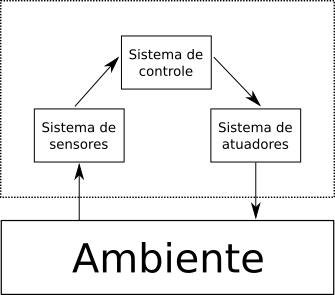
\includegraphics[width=0.5\textwidth, keepaspectratio]{sistemas_em_tempo_real}
    \centering
    \caption{Diagrama de um sistema em tempo real genérico. Adaptado de~\citeonline{BUTTAZZO:2011}}
    \label{fig:rt}
\end{figure}

% Existe um certo consenso na comunidade de que a evolução rápida no processamento de dados irá tornar a utilização de sistemas em tempo real obsoleta, no entanto tal afirmação não poderia estar mais enganada, apesar da 
Em termos de processamento, a computação mais rápida reduz o tempo de resposta de um sistema, entretanto ela não necessariamente garante que o tempo de resposta de tarefas individuais será atingido de maneira correta, um sistema em tempo real não deve apenas ser rápido, ele deve ser previsível. Analisando os sistemas do ponto de vista de processos, os processos de um sistema em tempo real contam com um componente ausente em processos de sistemas normais, o chamado \textit{Deadline}, que é o prazo máximo para a finalização de uma determinada tarefa.\cite{BUTTAZZO:2011}

Em aplicações críticas o retorno de operações fora do \textit{deadline} não é apenas atrasado, mas sim incorreto, o que pode ocasionar em perdas significativas dependendo da criticidade do sistema.~\cite{BUTTAZZO:2011} Em um contexto de um sistema de banco de dados de tempo real, a perda de deadlines pode acarretar em sobrecarregamentos em requisições ao banco de dados, o que tornaria o sistema inutilizável. \cite{bd:1991} A criticidade de uma aplicação depende das consequências ocasionadas devido ao atraso no tempo de resposta esperado do sistema, sendo este classificado em \textit{Hard}, \textit{Firm} e \textit{Soft}. \cite{BUTTAZZO:2011} 

\begin{itemize}
\item Sistemas críticos \textit{Hard} são aqueles onde caso não haja resposta no tempo definido podem ocorrer eventos devastadores, muitas vezes com perda de vidas;
\item Sistemas críticos \textit{Firm} são aqueles onde o atraso na resposta torna o sistema inútil, no entanto nenhum dano é gerado; e
\item Sistemas críticos \textit{Soft} são aqueles onde resultados após o tempo de resposta definido ainda tem alguma utilidade para o sistema, mesmo gerando perda de desempenho.
\end{itemize}


Usualmente os sistemas embarcados trabalham de maneira hibrida quanto a sua criticidade, onde certas atividades podem ser consideradas como \textit{Hard} e outras podem ser \textit{Soft} ou \textit{Firm}. Atividades com criticidade \textit{Hard} incluem: coleta de dados utilizando sensores, detecção de condições críticas, filtragem de dados, etc. Atividades que contam com com uma criticidade \textit{Firm} podem ser encontradas em aplicações de redes e multimídia, por exemplo: processamento de imagem \textit{on-line}, execução de vídeos e decodificação de áudio e vídeo. Já atividades com criticidade \textit{Soft} geralmente estão relacionadas à interação com o usuário como: a exibição de mensagens em uma tela, o processamento de sinais de teclado e o armazenamento de dados de utilização. \cite{BUTTAZZO:2011}

% A luva Hand.io é um sistema de tempo real que trabalha com atividades com criticidade \textit{Firm}, pois a falha no reconhecimento de um gesto e a realização da ação correspondente a este, não gera perdas de vidas ou perdas financeiras significativos, apenas tornam o sistema inútil.


%----------------------------------
% MICROS
%----------------------------------
\subsection{Microcontroladores e Microprocessadores}%ok

As diferenças entre microcontroladores e microprocessadores são apresentadas por \citeonline{ayala:1991} em seu livro, onde fica claro que apesar de terem surgido da mesma ideia e serem fabricados pelo mesmo grupo de pessoas, seu funcionamento e aplicação diferem grandemente. Existem diferenças fundamentais no design de tais dispositivos, enquanto microcontroladores por si só contam com todos os componentes necessários para o seu funcionamento, microprocessadores necessitam de outros componentes (exemplo, memória) e periféricos para funcionar como um computador completo.

Microprocessadores são conhecidos popularmente como Unidades Centrais de Processamento (CPU, em inglês), e tem como sua função principal buscar e modificar extensivamente dados da memória para que sejam armazenados ou exibidos para o usuário. Por si só um microprocessador não constitui um microcomputador completo, para se tornar uma máquina capaz de executar programas de propósito geral se faz necessária a utilização de memórias RAM, memórias de armazenamento massivo e diversos dispositivos de entrada e saída externos~\cite{ayala:1991}.

% O termo que melhor descreve 
Nos microprocessadores o hardware destes componentes é desenvolvido de tal maneira a permitir o desenvolvimento de sistemas grandes ou pequenos dependendo da demanda da aplicação. O projeto do microprocessador é desenvolvido de modo a atender as suas expectativas no mercado de consumo em massa.  
%\cite{ayala:1991}\todo{Apresentar um exemplo de microprocessador}.

Um exemplo de microprocessador seria o Broadcom BCM2837 \cite{raspberry_bcm}, que conta com quatro cores ARM que funcionam em uma frequência de $1.2$GHz. Este processador é encontrado no Raspberry Pi 3 \cite{raspberry:pi3}, exibido na \autoref{fig:raspberry}, que é um computador de placa única (SBC, em inglês). Por se tratar de um microprocessador, o Broadcom BCM2837 necessita de diversos outros componentes para funcionar como um computador completo.

\begin{figure}[ht]
    \centering
    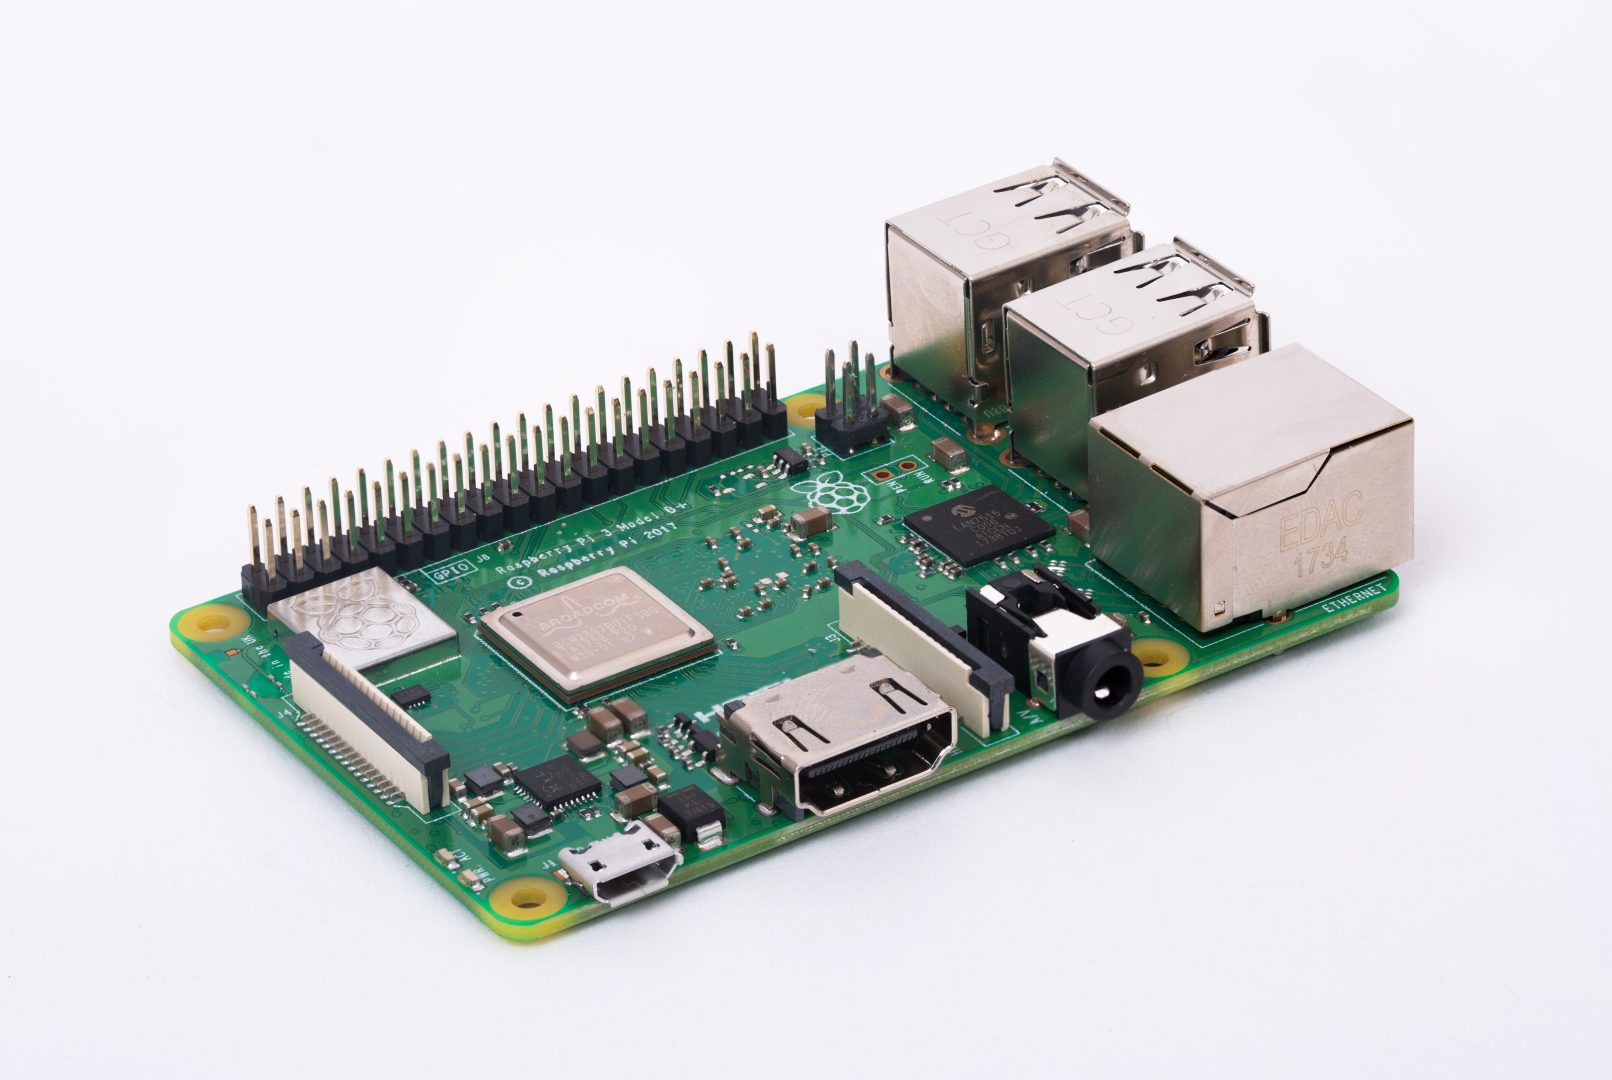
\includegraphics[width=0.5\textwidth, keepaspectratio]{resources/rasp.jpg}
    \caption{Raspberry Pi 3. \cite{raspberry:pi3}}
    \label{fig:raspberry}
\end{figure}

Os microcontroladores funcionam de maneira similar aos microprocessadores, no entanto, além de terem os componentes encontrados em um microprocessador eles também contam com todos os componentes necessários para o funcionamento de um computador completo, como memórias RAM, memórias ROM e portas paralelas e seriais de entrada e saída. Como os microprocessadores, os microcontroladores também são componentes de propósito geral, mas o seu foco deixa de ser apenas computar os dados encontrados na memória e armazená-los, e passa também controlar o ambiente em que se encontram se baseando nos resultados do processamento dos dados disponíveis \cite{ayala:1991}.

Os programas utilizados em microcontroladores são armazenados na memória ROM e não tem seu funcionamento alterado durante o ciclo de vida do sistema. As instruções de máquina encontradas nos microcontroladores geralmente envolvem buscar dados na memória interna e que também realizam operações envolvendo os pinos de conexão inclusos na plataforma, o que permite que cada pino tenha seu propósito programado de acordo com a vontade do desenvolvedor \cite{ayala:1991}

%\todo{Apresentar um exemplo de microcontrolador com a descrição da pinagem}.

Um exemplo de microcontrolador seria o ATmega328P~\cite{atmel}, apresentado na \autoref{fig:atmega},  que é o chip utilizado no Arduíno Uno \cite{arduino}. Por si só o ATmega328P conta com memória interna de 32 kilobytes para a gravação de programas de propósito geral, capacidade de controlar seus pinos e realizar cálculos complexos com os dados providos por eles. Quando integrado à uma placa de microcontrolador como o Arduíno o desenvolvimento passa a ser muito mais simplificado sendo necessário apenas um cabo micro USB para a gravação de programas na memória.

\begin{figure}[ht]
    \centering
    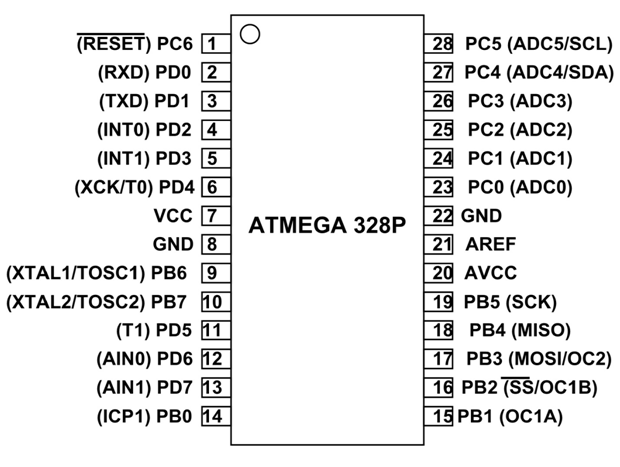
\includegraphics[width=0.7\textwidth, keepaspectratio]{resources/ATMega328P-Pinout.png}
    \caption{Pinagem do microcontrolador ATmega328P. \cite{atmel}}
    \label{fig:atmega}
\end{figure}

\todo[inline]{Sugiro explicar de forma curta a pinagem da \autoref{fig:atmega}}

%----------------------------------
% VSS
%----------------------------------

\section{Modelagem e verificação de sistemas}

Segundo \citeonline{edwards:1997}, os sistemas atualmente, em sua maioria, são desenvolvidos com uma abordagem \textit{ad hoc}, que é baseada em experiências prévias dos desenvolvedores com produtos similares aos que serão utilizados durante a implementação do sistema. Uma abordagem utilizando modelos formais e métodos de síntese automatizada de implementação é uma maneira mais efetivas de garantir um sistema seguro, visto que tais abordagens adotam modelos matemáticos para certificar propriedades de execução do sistema desenvolvido. 

Um modelo é uma representação abstrata e simplificada de uma coisa real. No desenvolvimento de sistemas um modelo permite aos desenvolvedores a possibilidade de distinguir o que realmente é necessário e o que é supérfluo, além de permitir que seja realizada uma análise mais rápida do sistema do que se cada componente do sistema tivesse que ser analisado individualmente \cite{UML:2006}.

A utilização de um ou mais modelos formais para descrever os comportamentos do sistema antes de tomar decisões mais específicas da implementação, como por exemplo, qual plataforma de hardware ou qual linguagem de programação utilizar, podem reduzir consideravelmente as falhas durante o funcionamento do sistema \cite{edwards:1997}.

Estes modelos permitem que as propriedades do sistema sejam validadas de maneira simples, ainda durante as fases inciais do desenvolvimento, através de ferramentas de simulação e verificação automatizadas, evitando eventuais entraves que podem comprometer a eficiência do sistema \cite{edwards:1997}.

% =============================
\subsection{United Modeling Language}
% =============================

De acordo com \citeonline{UML:2006} a Linguagem de Modelagem Unificada (UML, em Inglês) é um padrão amplamente utilizado por desenvolvedores para modelagem de software e hardware de sistemas em geral. A UML é uma ferramenta muito útil durante o desenvolvimento de um sistema, pois permite aos desenvolvedores manter um certo controle sobre a complexidade do sistema, permitindo que as partes mais importantes do sistema se sobressaiam em relação às outras, evitando eventuais confusões durante a implementação.

Por se tratar de uma linguagem formal, a UML permite a utilização de ferramentas de engenharia de sistemas auxiliada por computador (CASE, em inglês) que geram código executável a partir dos diagramas de modelagem do sistema. Existem diferentes maneiras de utiliza a UML, alguns desenvolvedores a utilizam como um esboço do sistema frisando os componentes mais importantes para a implementação, alguns utilizam como planta baixa do sistema mantendo qualquer mudança realizada no código sincronizada com os modelos e outros utilizam como linguagem de programação, graças à natureza orientada a objetos da UML a conversão de diagramas em código de máquina passa a ser uma realidade no cotidiano de alguns desenvolvedores. \cite{UML:2006}

Diversos diagramas são utilizados para a especificação de um sistema. Cada um deles sendo utilizado para descrever alguma parte do modelo, sem conter informações demais relacionadas à outras partes do projeto o que poderia causar confusão durante a implementação do sistema. Abaixo estão listados os diagramas UML e suas respectivas funções. \cite{UML:2006}.

\begin{itemize}
    \item \textbf{Diagrama de caso de uso:} utilizado para modelar interações entre usuário e sistema, também sendo usado para levantamento de requisitos.
    \item \textbf{Diagrama de atividade:} utilizado para modelar atividades sequenciais e paralelas do sistema.
    \item \textbf{Diagrama de classe:} utilizado para modelar classes, tipos, interfaces e as relações entre eles.
    \item \textbf{Diagrama de objeto:} utilizado para modelar as instâncias das classes definidas no diagrama de classes.
    \item \textbf{Diagrama de sequência:} utilizado para modelar as interações entre objetos quando a ordem delas é importante.
    \item \textbf{Diagrama de comunicação:} utilizado para modelar a maneira como os objetos interagem e as conexões necessárias para as interações.
    \item \textbf{Diagrama de tempo:} utilizado para modelar as interações entre objetos quando o tempo é uma preocupação importante
    \item \textbf{Diagrama de visão geral de interação:} utilizado para unir os diagramas de sequencia, comunicação e tempo com a finalidade de ter uma visão geral do sistema. 
    \item \textbf{Diagrama de estrutura composta:} utilizado para modelar os componentes internos de uma classe e descrever as relações entre objetos em uma dada situação.
    \item \textbf{Diagrama de componente:} utilizado para modelar os componentes importantes do sistema e as interfaces que eles utilizam para comunicação;
    \item \textbf{Diagrama de pacote:} utilizado para descrever a organização hierárquica de grupos de classes e componentes.
    \item \textbf{Diagrama de estados:} utilizado para modelar o estado de um objeto durante seu período de vida e os eventos que podem gerar mudanças de estados.
    \item \textbf{Diagrama de implantação:} utilizado para descrever como um sistema pode ser implantado em uma situação real.
\end{itemize}

Os diagramas UML, em especial o diagrama de sequência, podem descrever com precisão as interações que ocorrem durante o funcionamento de um sistema embarcado \cite{uml_petri}. Existem ferramentas como o FOREVER \cite{forever} que podem gerar redes de Petri a partir de um diagrama de sequência, o que pode auxiliar grandemente a verificação automatizada do comportamento de um sistema.

%\todo[inline]{Apresentar os diagramas com exemplo}

\todo[inline]{Apresentar um exemplo usando FOREVER \cite{forever}}

%\todo[inline]{Descrever um exemplo com diagrama de sequência e apresentar como será usado no seu TCC}

% \subsection{Modelos Formais}

% =============================
\subsection{Máquina de Estados}
% =============================

Segundo \citeonline{hopcroft:2001} máquinas de estados finitos, também conhecidas como autômatos finitos, são uma maneira muito útil e visual de modelar o comportamento de um sistema de maneira que seus componentes ou subsistemas estejam sempre realizando um conjunto de tarefas finitas que podem ser representadas e rastreadas através de estados que são alterados em resposta à entradas externas. 

De acordo com \citeonline{hopcroft:2001}, formalmente uma máquina de estados finitos é definida por uma quíntupla $A = (Q, \Sigma, \delta, q_0, F)$ onde:

\begin{itemize}
    \item $Q$ é um conjunto de estados.
    \item $\Sigma$ é um conjunto finito de símbolos de entrada.
    \item $\delta$ é uma função de transição que recebe um estado e um símbolo e retorna um outro estado.
    \item $q_0$ é um estado inicial que faz parte de $Q$
    \item $F$ é um conjunto estados finais que é subconjunto de $Q$ 
\end{itemize}

Existem duas grande categorias de máquinas de estados, as determinísticas, onde apenas um estado é atingido por vez, e não determinísticas, que permite que vários estados podem estar sendo acessados ao mesmo tempo. \cite{hopcroft:2001}

Um exemplo de modelagem de sistemas com máquinas de estados finitos seria a modelagem de uma máquina de doces com troco automático apresentada por \cite{snack} na \autoref{fig:snack}\todo{Adicionar um breve explicação da figura}.

\begin{figure}[ht]
    \centering
    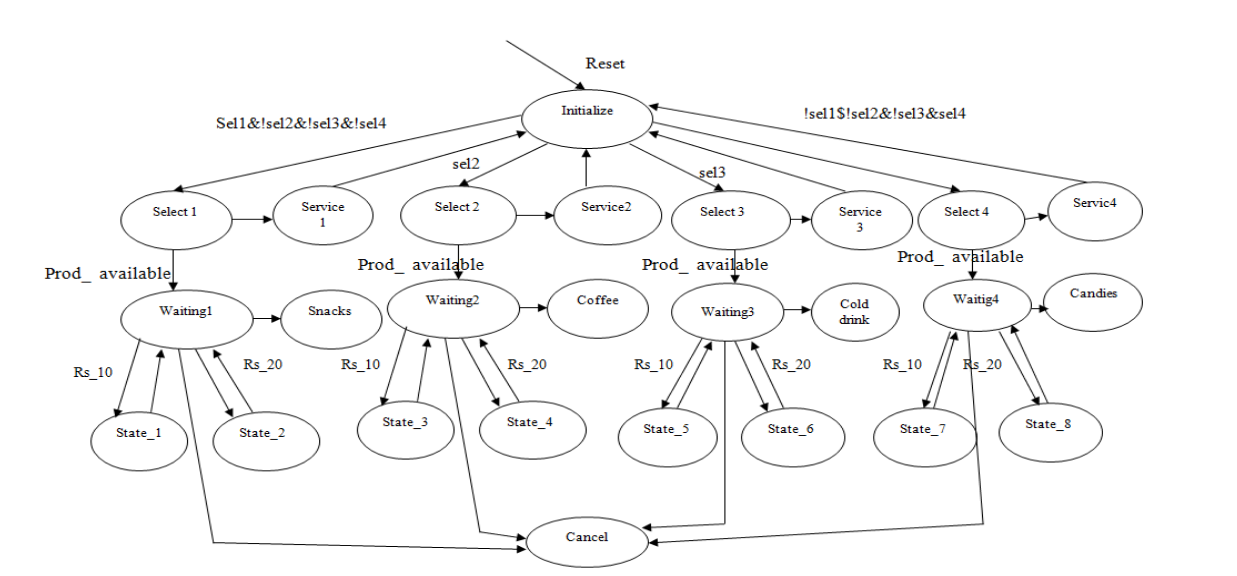
\includegraphics[width=\textwidth, keepaspectratio]{resources/snackmachine.png}
    \caption{Máquina de estados finita da máquina de venda de doces. \cite{snack}}
    \label{fig:snack}
\end{figure}

 \newpage
%\todo[inline]{Descrever os tipos de máquina de estado}

%\todo[inline]{Apresentar um exemplo de modelagem de sistema usando máquina de estado.}

% O propósito do estados é que o sistema tenha noção do seu histórico, se lembrando apenas das partes relevantes.



\subsection{Rede de Petri}
\label{def:petri_prop}
\citeonline{murata:1989} apresenta redes de Petri como uma ferramenta de modelagem de sistemas visual e matemática, que pode ser aplicada em diversas áreas de conhecimento, desde modelagem de grande linhas de produção até para avaliação de desempenho em sistemas com lógica sequencial ou paralela. Por se tratar de um modelo matemático, as redes de Petri podem ser utilizadas em conjunto com ferramentas de teste automatizado para analisar se o sistema modelado está funcionando de maneira correta.


\begin{table}[ht]
    \centering
    \begin{tabular}{|l|}
         \hline
         Formalmente uma rede de Petri é uma quíntupla, $PN = (P,T,F,W,M_0)$ onde: \\ \hline
         $P = \{p_1,p_2,\ldots,p_m\}$ é um conjunto finito de lugares, \\
         $T = \{t_1,t_2,\ldots,t_n\}$ é um conjunto de transições, \\
         $F \subseteq (P \times T) \cup (T \times P)$ é um conjunto de arcos, \\
         $W: F \to \{1,2,3,\ldots\} $ é uma função de pesos, \\
         $M_0: P \to \{0,1,2,3,\ldots\}$ é a marcação inicial, \\
         $P \cap T = \emptyset$ e $P \cup T \neq \emptyset$ \\
         Uma rede de Petri sem qualquer marcações iniciais é denominada por $N$ \\
         \hline
    \end{tabular}
    \caption{Definição formal de uma rede de Petri. Adaptada de \citeonline{murata:1989}.}
    \label{tab:petri_form}
\end{table}

As mudanças pelas quais o sistema passa durante seu funcionamento são simuladas em uma rede de Petri seguindo regras de transição, exemplificado na \autoref{fig:petri}, onde na letra $(a)$, a transição $t$ pode ser ativada quando os lugares $H_2$ e $O_2$ conterem marcações chamadas de \textit{tokens}, representados por círculos pretos, suficientes para ultrapassar o peso $w$ correspondente à um arco $f$ que liga $H_2$ e $O_2$ até $t$. Após a ativação da transição $t$, apresentada na letra $(b)$, são removidos a quantidade de \textit{tokens} dos lugares $H_2$ e $O_2$ iguais ao peso $w$ que incide em $t$, e então são adicionados a quantidade de \textit{tokens} correspondentes ao peso $w$ do arco que liga $t$ à $H_2O$ \cite{murata:1989}.

\begin{figure}[ht]
    \centering
    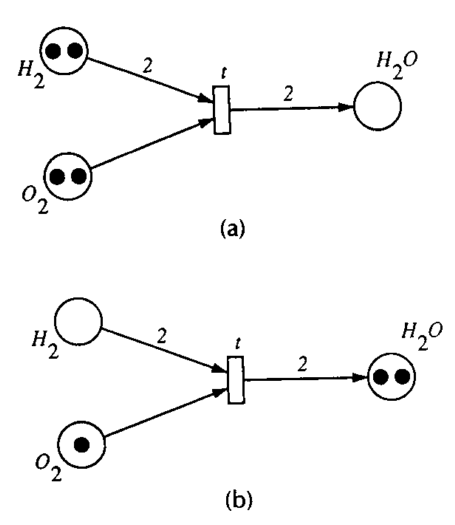
\includegraphics[width=0.4\textwidth, keepaspectratio]{resources/petri.png}
    \caption{Regra de transição. \cite{murata:1989}}
    \label{fig:petri}
\end{figure}

Um exemplo de uma rede de Petri modelando um sistema real pode ser apresentado na \autoref{fig:petri_ex}, onde o funcionamento de uma máquina de doce simples está descrito em detalhes\todo{Apresentar um breve explicação}.

\begin{figure}[ht]
    \centering
    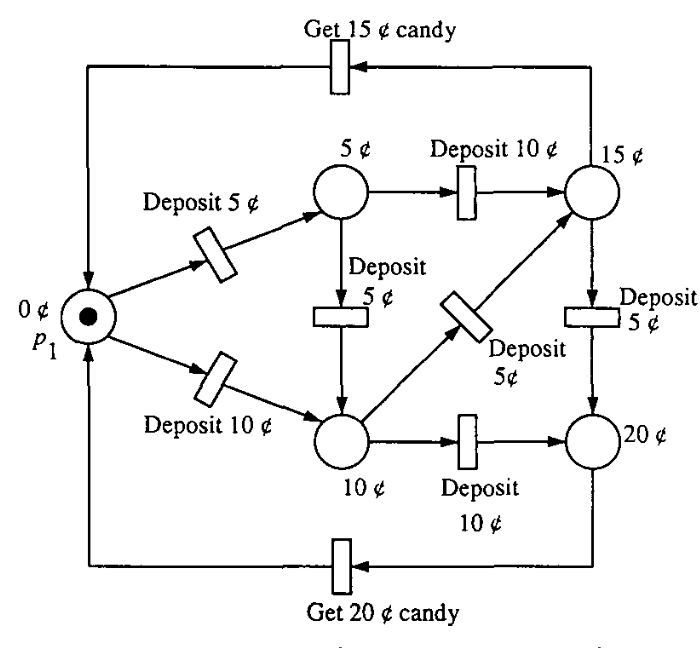
\includegraphics[width=0.4\textwidth, keepaspectratio]{resources/petriexemplo.png}
    \caption{Modelagem de uma máquina de doce utilizando rede de Petri. \cite{murata:1989}}
    \label{fig:petri_ex}
\end{figure}

Segundo \citeonline{peterson:1981} existem algumas propriedades que uma rede de Petri devem ser atendidas para que não ocorram eventuais problemas durante o funcionamento do sistema modelado. Seguem elas listadas a baixo:


\begin{itemize}
    \item \textbf{Segurança:} uma rede de Petri é tida como segura quando em nenhum momento existem mais de um \textit{token} por lugar. 
    \item \textbf{Limitação:} uma rede de Petri atende as propriedades de limitação quando o numero de \textit{tokens} não excede um limite $k$ definido pelo desenvolvedor.
    \item \textbf{Conservação:} uma rede de Petri atende as propriedades de conservação quando existe uma quantidade fixa de \textit{tokens} em todos os momentos do seu funcionamento.
    \item \textbf{Vivacidade:} uma rede de Petri cumpri as propriedades de vivacidade quando não ocorrem travas durante o seu funcionamento devido à má utilização de \textit{tokens}.
\end{itemize}





%\todo[inline]{Definir formalmente, e apresentar um exemplo prático.}



%----------------------------------
% IoT
%----------------------------------
\section{Internet das Coisas}

No trabalho de~\citeonline{ATZORI:2010} é demonstrado que em sua ideia fundamental a internet das coisas é um ambiente de computadores pervasivos que interagem um com os outros de maneira cooperativa para atingir metas em comum, este conceito permite a idealização de ambientes inteligentes onde todos os objetos estão em constante comunicação: para auxiliar o usuário a atingir uma qualidade de vida maior.

Nos ambientes residenciais e empresariais, a internet das coisas pode tornar a vida muito mais confortável e eficiente com sensores e atuadores, coletando dados sobre a preferência dos usuários e sobre o clima é possível que a temperatura seja adequada automaticamente levando em consideração o gasto de energia elétrica para uma maior economia. \cite{ATZORI:2010}

% \begin{comment}
% \begin{figure}
%     \centering
%     \includegraphics{}
%     \caption{Sensores e atuadores em IoT}
%     \label{fig:my_label}
% \end{figure}
% 
% \end{comment}

\todo[inline]{Adicionar uma figura exemplificando os sensores e atuadores em IoT}

%----------------------------------
% IA
%----------------------------------
\section{Reconhecimento de Padrões}

Segundo \citeonline{bishop:2006} o problema de encontrar padrões em dados é um problema famoso e antigo que desde sempre intrigou cientistas mundo a fora. A observação de padrões na natureza serviu de fundação para a criação de modelos matemáticos que servem de base para a física moderna que até hoje é utilizada para para resolver problemas reais. 

Atualmente o campo de reconhecimento de padrões é focado na identificação automática de regularidades em grandes conjuntos de dados, utilizando algoritmos computadorizados. Os resultados destes algoritmos podem ser utilizados para classificar estas regularidades em diferentes grupos. \cite{bishop:2006}. Vale ressaltar que com o uso de sistema em IoT uma grande quantidade de dados é gerado pelos sensores adotados, logo técnicas de reconhecimento de padrões podem ser uma solução para classificar e prever determinadas ações nestes sistemas.

\subsection{Aprendizagem de Máquina}

Segundo \citeonline{norvig:780391} o aprendizado ocorre quando um agente, seja ele uma máquina ou um humano, melhora seu desempenho em tarefas futuras após realizar observações do ambiente no qual ele atua se baseando em pares de entradas e saídas para prever novas saídas a partir de novas entradas.

A utilização do aprendizado de máquina se justifica pela necessidade de criar sistemas adaptativos, pois durante o desenvolvimento muitas vezes não é possível prever mudanças que podem ocorrer no ambiente no qual o sistema irá atuar, ou mesmo porque não é possível de maneira simples desenvolver um sistema que possa atender as necessidades da aplicação utilizando métodos tradicionais de programação \cite{norvig:780391}.

De acordo com \citeonline{norvig:780391} existem três tipos de aprendizado que diferem no tipo de \textit{feedback} informado ao agente que busca se aprimorar. No aprendizado não-supervisionado o agente busca aprender padrões nas entradas de dados sem que qualquer tipo de \textit{feedback} seja informado de maneira explícita. O tipo mais comum de atividade deste tipo de aprendizado seria a criação de grupos a partir de entradas, por exemplo, um cachorro pode desenvolver uma noção sobre dias de passear ou dias de ficar em casa de acordo com o clima do dia sem que o seu dono tenha explicitamente dito que era a hora de passear.

No aprendizado por reforço o agente aprende a partir de incentivos ou punições que são aplicados de acordo com o resultado da predição de saídas a partir de novas entradas. Um exemplo deste tipo de aprendizado seria quando o dono de um cachorro tenta ensinar novos truques a ele oferecendo um biscoito quando ele realiza o truque de maneira correta, e falando com uma voz mais firme sem oferecer o biscoito quando ele realiza o truque de maneira incorreta. \cite{norvig:780391}

No aprendizado supervisionado, o agente observa pares de entradas e saídas e tenta criar novas funções para reproduzir estes resultados a partir de novas entradas. Um exemplo deste tipo de aprendizado acontece quando uma criança é ensinada sobre como realizar cálculos matemáticos simples e o professor apresenta exemplos de cálculos corretos esperando que a criança realize o mesmo cálculo com valores diferentes e resultados diferentes por si só, sendo informada se o resultado estava correto ou não \cite{norvig:780391}.

Um exemplo da aplicabilidade de algoritmos de aprendizado de máquina seria o reconhecimento de escrita. Devido a grande variedade de tipos de escrita, este problema conta com um alto grau de complexidade de implementação. Para este problema é utilizada uma imagem de $28$ por $28$ pixeis como representação de um caractere escrito a mão, que é apresentada para o algoritmo como um vetor composto por $784$ números reais. A criação de um algoritmo utilizando heurísticas e regras feitas para casos específicos acabaria criando um grande volume de regras e exceções o que levaria a resultados ruins no reconhecimento. \cite{bishop:2006}

Resultados melhores podem ser atingidos utilizando algoritmos de aprendizado de máquina. Um grande volume de dígitos escritos a mão representados por um conjunto de vetores e um vetor com valores representando categorias manualmente escolhidas por um desenvolvedor são conhecidos como \textit{training sets}, e são utilizados como referência para a realização de ajustes nos parâmetros de um algoritmo de aprendizado de máquina. A ideia por trás deste método é que o algoritmo passe a categorizar novos vetores que não fazem parte do \textit{training set} original nas categorias definidas previamente. A habilidade de reconhecer estes novos padrões corretamente é conhecida como \textit{generalização} \cite{bishop:2006}.

\subsection{\textit{Frameworks} de aprendizado de máquina}

Como o foco deste trabalho não é o desenvolvimento e a implementação de algoritmos de aprendizado de máquina, serão utilizados \textit{frameworks} desenvolvidos em Python prontos para desenvolvimento. 

\subsubsection{Scikit-learn}

O \textit{Scikit-learn} é um módulo de código aberto para a linguagem \textit{Python} que conta com implementações do estado da arte de diversos algoritmos de aprendizado de máquina para análise de grandes volumes de dados. Por contar com código compilado a execução dos algoritmos acontece de maneira muito mais rápida que em outras plataformas \textit{Python} que utilizam interpretadores para realizar cálculos complexos. \cite{scikit-learn} 

Graças à sua API simples integrada à linguagem \textit{Python}, o \textit{Scikit-learn} pode ser utilizado por diversos profissionais de diversas áreas sem conhecimentos avançados da implementação de algoritmos de aprendizado de máquina. A natureza padronizada da implementação dos algoritmos, permite que comparações de desempenho sejam facilmente realizadas. Algoritmos que são tidos como padrões na industria como a \textit{SVM} \cite{cortes:1995svm}, \textit{kNN} \cite{cover:1967knn} e \textit{k-means} \cite{macqueen:1967kmeans} estão implementados no módulo. \cite{scikit-learn}

\todo[inline]{Adicionar exemplo}

\subsubsection{Tensoflow}

O TensorFlow é uma plataforma de aprendizado de máquina de código aberto desenvolvida por \citeonline{tensorflow:2016}, possibilita ao desenvolvedor realizar o treinamento de um algoritmo em uma plataforma extremamente escalável podendo ser utilizado tanto em grandes \textit{clusters} de servidores quanto em dispositivos móveis. As computações sendo realizadas no algoritmo e o estado no qual este se encontra podem ser visualizadas em tempo real através de uma interface visual em alto nível. Tal interface permite ao desenvolvedor tomar decisões rápidas sobre como otimizar o algoritmo que está sendo treinado.

\todo[inline]{Ampliar descrição e Adicionar exemplo}

